\documentclass[12pt]{report}
\usepackage[utf8]{inputenc}
\usepackage{graphicx}     % For including images
\usepackage{subcaption}   % For subfigure environment
\usepackage{hyperref}
\usepackage{geometry}
\usepackage{float}
\usepackage{titlesec}
\usepackage{setspace}
\usepackage{fancyhdr}
\usepackage{array}
\usepackage{enumitem}
\usepackage{listings}   % For code listings
\usepackage{tcolorbox}  % For colored boxes
\tcbuselibrary{listings} % Integrate listings with tcolorbox
\usepackage{booktabs}   % For professional quality tables
\usepackage{tabularx}   % For tables with adjustable-width columns
\usepackage{longtable}  % For tables that span multiple pages
\usepackage{times}

% Page geometry
\geometry{
    a4paper,
    left=1in,
    right=1in,
    bottom=1in,
    includefoot
}

% Set line spacing to 1.5
\onehalfspacing

% Format headings
\titleformat{\chapter}[display]
  {\normalfont\fontsize{18}{22}\bfseries}
  {}
  {-30pt}  % <-- Reduces the space BEFORE the title
  {\centering\MakeUppercase}
\titlespacing*{\chapter}{0pt}{-40pt}{20pt}  % <-- {left}{before-sep}{after-sep}


\titleformat{\section}
  {\normalfont\fontsize{16}{19}\bfseries}{\thesection}{1em}{}

\titleformat{\subsection}
  {\normalfont\fontsize{14}{17}\bfseries}{\thesubsection}{1em}{}

% Set normal text size to 12pt Times New Roman
\renewcommand{\normalsize}{\fontsize{12}{14}\selectfont}

% Title page style
\fancypagestyle{empty}{
    \fancyhf{}
    \renewcommand{\headrulewidth}{0pt}
    \renewcommand{\footrulewidth}{0pt}
}

% Ensure chapter pages use plain style
\renewcommand{\chapterpagestyle}{plain}

\renewcommand{\maketitle}{
    \begin{titlepage}
        \centering
        \vspace*{-2cm}
        
        % Logo and College Name with header
        \begin{center}
            \includegraphics[width=1.025\textwidth]{images/rvce_logo_header_2.jpg}\par
        \end{center}
        \vspace{0.5cm}
        
        % Department
        {\Large\bfseries DEPARTMENT OF INFORMATION SCIENCE AND ENGINEERING\par}
        \vspace{0.7cm}

        % Theme and Title
        {\large\bfseries Title: IoT-Based Vital Sign Monitoring System with Conversational Health Data Access\par}
        \vspace{1cm}
        
        % Lab Report Title
        {\Large\bfseries IoT and Applications\par}
        \vspace{0.3cm}
        {\large IS237DL\par}
        \vspace{0.7cm}
        
        % Submitted by
        {\large\bfseries Submitted by\par}
        \vspace{0.3cm}
        \begin{tabular}{ll}
            Avinash Anish 1RV23IS145  \\ 
            \hspace{0.35cm} Disha A 1RV23IS402 \\
            Kotra Sasank 1RV23IS062 \\
        \end{tabular}
        \vspace{1cm}
        
        % Guide
        {\large\bfseries Under the guidance of\par}
        \vspace{0.2cm}
        Prof. Sushmitha N \\
        Assistant Professor\\
        Dept. of ISE\\
        RV College of Engineering®\par
        \vfill
        
        % Academic Year
        {\large 2024-2025}
    \end{titlepage}
}

\title{\fontsize{16}{19}\selectfont IoT-Based Vital Sign Monitoring System with Conversational Health Data Access}
\author{Department of Information Science and Engineering\\
        RV College of Engineering}
\date{\today}

\begin{document}

\maketitle
\newpage

% Abstract (kept as per original, can be moved or removed by user)
\begin{abstract}
This paper presents HealthHub, an AI-powered personal health assistant designed to help individuals make informed daily dietary choices by providing personalized food safety and nutritional insights. Users can log food intake, which HealthHub analyzes using a Retrieval-Augmented Generation (RAG) pipeline to query diverse sources like FSSAI advisories and food databases, and an SQL agent for nutritional pattern analysis. The system uniquely integrates personal health sensor data (e.g., heart rate) to correlate diet with physiological responses, offering potential risk warnings. HealthHub features an intuitive voice and video-enabled interface, aiming to empower users with accessible, actionable information for enhanced food safety awareness and personal well-being. Performance evaluations highlight the system's capability in processing user queries effectively and integrating multimodal data for comprehensive dietary support.
\end{abstract} 
\newpage

\tableofcontents
\newpage

\chapter{Introduction to IoT-Based Vital Sign Monitoring System with Conversational Health Data Access}
% Chapter 1: Introduction to IoT-Based Vital Sign Monitoring System with Conversational Health Data Access
% This section should contain the use of the project in real time, as per the provided guidelines.

\section*{Introduction}
Your introduction content goes here.


\chapter{Existing System Study and its Outcome with Project Objectives}
\section{IoT-Based Health Monitoring Systems}

\begin{enumerate}
    \item Remote Patient Monitoring Systems
    \begin{itemize}
        \item Commercial solutions like Philips HealthSuite Digital Platform and Medtronic CareLink provide continuous monitoring but typically lack conversational interfaces
        \item Most systems require healthcare provider interpretation of data
        \item Limited personalization capabilities for individual user needs
    \end{itemize}

    \item Wearable Health Trackers
    \begin{itemize}
        \item Consumer devices (Fitbit, Apple Watch, Samsung Galaxy Watch) offer basic vital sign monitoring
        \item Typically monitor limited parameters (heart rate, activity, sometimes ECG)
        \item Data presentation is primarily visual/graphical with minimal natural language interpretation
        \item Users often struggle to contextualize the health significance of their data
    \end{itemize}

    \item Smart Home Health Monitoring
    \begin{itemize}
        \item Smart home platforms integrating health devices (Amazon Alexa + Omron blood pressure monitor)
        \item Basic voice command capabilities but limited to simple queries
        \item Lack comprehensive vital sign integration and contextual health understanding
    \end{itemize}
\end{enumerate}

\section{Conversational Health Interfaces}

\begin{enumerate}
    \item Healthcare Chatbots
    \begin{itemize}
        \item Systems like Ada Health, Babylon Health, and Buoy Health provide symptom assessment
        \item Focus primarily on diagnostic information rather than personal health data interpretation
        \item Limited integration with real-time physiological monitoring devices
        \item Typically use rule-based approaches rather than advanced NLP techniques
    \end{itemize}

    \item Voice Assistants in Healthcare
    \begin{itemize}
        \item Voice-enabled systems (Alexa Skills for healthcare, Google Assistant healthcare actions)
        \item Capabilities include medication reminders, appointment scheduling, and basic health information
        \item Limited in processing and contextualizing continuous health data streams
        \item Privacy concerns with cloud-based processing of sensitive health information
    \end{itemize}

    \item Natural Language Understanding in Health Data
    \begin{itemize}
        \item Research systems employing NLP for electronic health records (EHRs)
        \item Focus on clinical documentation rather than consumer-facing applications
        \item Limited capabilities for real-time data processing from IoT devices
        \item Few systems combine IoT sensor data with conversational interfaces
    \end{itemize}
\end{enumerate}

\section{Key Limitations}

\begin{enumerate}
    \item Integration Challenges
    \begin{itemize}
        \item Most solutions either focus on robust IoT monitoring OR natural language interfaces, rarely both
        \item Limited interconnectivity between sensing devices and conversational systems
        \item Data silos prevent comprehensive health insights
    \end{itemize}

    \item Technical Complexity
    \begin{itemize}
        \item Existing systems often require technical expertise to install, configure and interpret
        \item Complex user interfaces create barriers for elderly or non-technical users
        \item Data visualization without context-aware explanations limits usefulness
    \end{itemize}

    \item Limited Personalization
    \begin{itemize}
        \item Generic health advice rather than personalized insights based on individual data patterns
        \item Minimal adaptation to user's health literacy level or communication preferences
        \item One-size-fits-all approaches to data presentation and interaction
    \end{itemize}

    \item Privacy and Security
    \begin{itemize}
        \item Centralized data storage raising privacy issues
        \item Limited transparency in how health data is processed and stored
        \item Inadequate security measures for sensitive personal health information
    \end{itemize}

    \item RAG Limitations
    \begin{itemize}
        \item Few systems leverage RAG capabilities for personalized health information retrieval
        \item Limited contextual understanding when processing natural language queries about health data
        \item Lack of integration between personal health data repositories and language models
    \end{itemize}
\end{enumerate}

\begin{figure}[h!]
    \centering
    \includegraphics[width=\textwidth]{images/lr2.png}
    \caption{Literature review comparison of existing systems (Part 1)}
\end{figure}

\begin{figure}[h!]
    \centering
    \includegraphics[width=\textwidth]{images/lr3.png}
    \caption{Literature review comparison of existing systems (Part 2)}
\end{figure}
\section{OBJECTIVES}

\begin{enumerate}
    \item \textbf{To Build an IoT Health Monitoring System}
    \begin{itemize}
        \item Set up Arduino-based sensors for ECG, heart rate, pulse, and temperature monitoring
        \item Create a system to collect real-time vital sign data
        \item Design a dashboard to display live health measurements
    \end{itemize}

    \item \textbf{To Create a Natural Language Interface}
    \begin{itemize}
        \item Develop a conversational system using LLM models
        \item Enable users to ask questions about their health data in simple language
        \item Provide easy-to-understand responses to health data queries
    \end{itemize}

    \item \textbf{To Make Health Data Easy to Understand}
    \begin{itemize}
        \item Convert complex health readings into simple explanations
        \item Create visual representations of health trends
        \item Provide personalized health insights based on collected data
    \end{itemize}

    \item \textbf{To Ensure Data Safety and Privacy}
    \begin{itemize}
        \item Protect user health data through encryption
        \item Follow healthcare data protection rules
        \item Create secure ways to store and access health information
    \end{itemize}
\end{enumerate}

\chapter{Project Architecture \& Design}
\section{System Architecture and Design}

\subsection{System Architecture Overview}

The system architecture comprises a modular IoT-based health monitoring framework integrated with a cloud backend and an AI-powered frontend interface. The architecture includes microcontrollers, biomedical sensors, communication modules, a database, backend APIs, and a real-time frontend dashboard. Sensor data is transmitted via Wi-Fi to a cloud database where it is processed, visualized, and queried using natural language.

\begin{figure}[h!]
\centering
\includegraphics[width=\textwidth]{images/feature_implementation.png}
\caption{System Architecture Diagram}
\end{figure}

\subsection{Hardware Components and Configuration}

\textbf{Components and Sensors Used:}

\begin{itemize}
    \item \textbf{Microcontroller:}
    \begin{itemize}
        \item \textbf{Arduino UNO R3} – Acts as the core controller for sensor interfacing and data collection.
    \end{itemize}

    \item \textbf{Wi-Fi Module:}
    \begin{itemize}
        \item \textbf{ESP8266} – Ensures wireless connectivity and enables real-time data transfer to the backend.
    \end{itemize}

    \item \textbf{Biomedical Sensors:}
    \begin{itemize}
        \item \textbf{MAX30102} – Captures \textbf{SpO2} and \textbf{heart rate} data using IR and red LED photodetectors.
        \item \textbf{AD8232} – Acquires real-time \textbf{ECG signals}, enabling heart activity tracking through electrode pads.
        \item \textbf{SEN-11574} – Detects \textbf{heartbeats} through finger contact with analog output.
        \item \textbf{LM35} – Measures \textbf{body temperature} with high accuracy via linear voltage output.
    \end{itemize}

    \item \textbf{Display Module:}
    \begin{itemize}
        \item \textbf{OLED Display (e.g., SSD1306)} – Visual feedback module for showing sensor values in real-time.
    \end{itemize}
\end{itemize}

\begin{figure}[h!]
\centering
\includegraphics[width=\textwidth]{images/sensor_integration.png}
\caption{IoT Sensor Setup and Configuration}
\end{figure}

\subsection{Technology Stack}

\textbf{Tech Stack Overview:}

\begin{itemize}
    \item \textbf{Hardware:} Arduino UNO R3, ESP8266, MAX30102, AD8232, LM35, SEN-11574, OLED Display
    \item \textbf{Firmware:} Arduino IDE (C++), sensor-specific libraries
    \item \textbf{Backend:} FastAPI, PostgreSQL (Supabase), MQTT/HTTP protocol
    \item \textbf{Frontend:} Next.js, TailwindCSS, shadcn/ui, Chart.js or Recharts
    \item \textbf{AI/NLP:} OpenAI GPT-4, LangChain, LangGraph, Cohere (for embeddings)
    \item \textbf{Storage \& Auth:} Supabase (Auth, RLS, pgvector for embeddings, file storage)
\end{itemize}

\subsection{Circuit Diagrams and Pin Configurations}
% Please add relevant circuit diagrams and pin configuration details here.
% Example: \begin{figure}[h!]
% \centering
% \includegraphics[width=0.8\textwidth]{images/circuit_diagram.png}
% \caption{Overall Circuit Diagram}
% \end{figure}

% Pin connections for Arduino UNO R3:
% - MAX30102: SDA -> A4, SCL -> A5
% - AD8232: OUTPUT -> A0, LO+ -> D10, LO- -> D11
% - ... and so on for other sensors and modules.


\chapter{Methodology for IoT-Based Vital Sign Monitoring System with Conversational Health Data Access}
\section{METHODOLOGY}

\subsection{Implementation Tasks}

\begin{enumerate}

\item \textbf{Frontend Development}
\begin{itemize}
    \item Design the user interface using \textbf{Next.js} with \textbf{TailwindCSS} and \textbf{shadcn/ui} for a responsive, modular experience.
    \item Build a real-time dashboard to visualize health metrics such as SpO2, heart rate, ECG, and temperature.
    \item Integrate Supabase Auth to enable secure user login and session handling.
\end{itemize}

\item \textbf{Backend Development}
\begin{itemize}
    \item Set up a \textbf{FastAPI} server to handle incoming sensor data and expose RESTful endpoints.
    \item Use a \textbf{PostgreSQL} database (hosted via Supabase) to store and manage health data securely.
    \item Develop APIs for data submission, retrieval, and query handling.
\end{itemize}

\item \textbf{IoT Sensor Integration}
\begin{itemize}
    \item Use an \textbf{Arduino UNO R3} to interface with all biomedical sensors and read analog/digital inputs.
    \item Employ an \textbf{ESP8266 Wi-Fi module} to transmit data to the cloud via HTTP or MQTT.
    \item Configure periodic data sampling and preprocessing before cloud transmission.
\end{itemize}

\item \textbf{AI Integration}
\begin{itemize}
    \item Integrate a conversational AI interface using \textbf{LangChain} and \textbf{GPT-4/GPT-4o}.
    \item Allow users to query their health records through natural language using a Text-to-SQL pipeline.
    \item Provide automated health summaries and anomaly detection powered by AI.
\end{itemize}

\end{enumerate}


\chapter{Results of IoT-Based Vital Sign Monitoring System with Conversational Health Data Access}
\section{Results}

This section presents the key outcomes from the development and initial testing of the HealthHub platform. We focused on evaluating the core functionalities, user interface effectiveness, and the performance of the AI-driven food safety and nutritional analysis features, particularly those concerning FSSAI guidelines and personal health data.

\subsection{User Interface and Experience}
HealthHub provides a clean and intuitive user interface, designed to make complex health and food safety information accessible. Figure \ref{fig:hm-hero} showcases the platform's landing page, introducing users to HealthHub's capabilities.

\begin{figure}[!t]
\centering
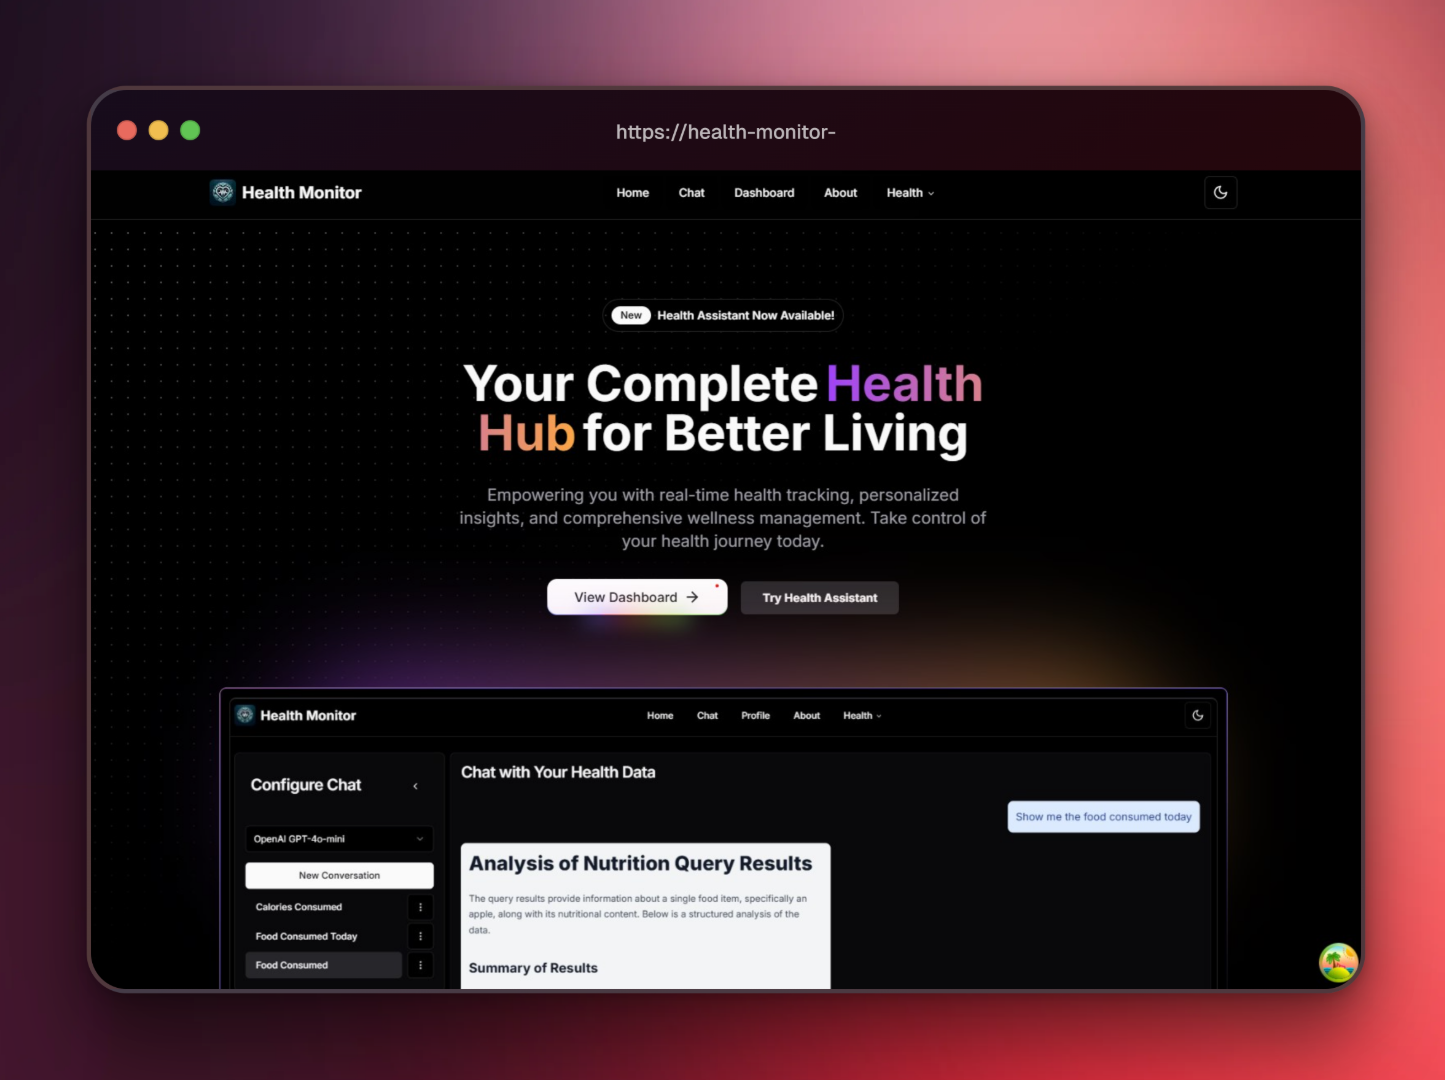
\includegraphics[width=0.9\columnwidth]{figures/hm-hero.png} % User to confirm/update path
\caption{The HealthHub landing page, highlighting its core features and value proposition to the user.}
\label{fig:hm-hero}
\end{figure}

Upon logging in, users are presented with the main dashboard (Figure \ref{fig:hm-dashboard}), which offers an overview of their logged data and quick access to various features, including food logging and initiating queries.

\begin{figure}[!t]
\centering
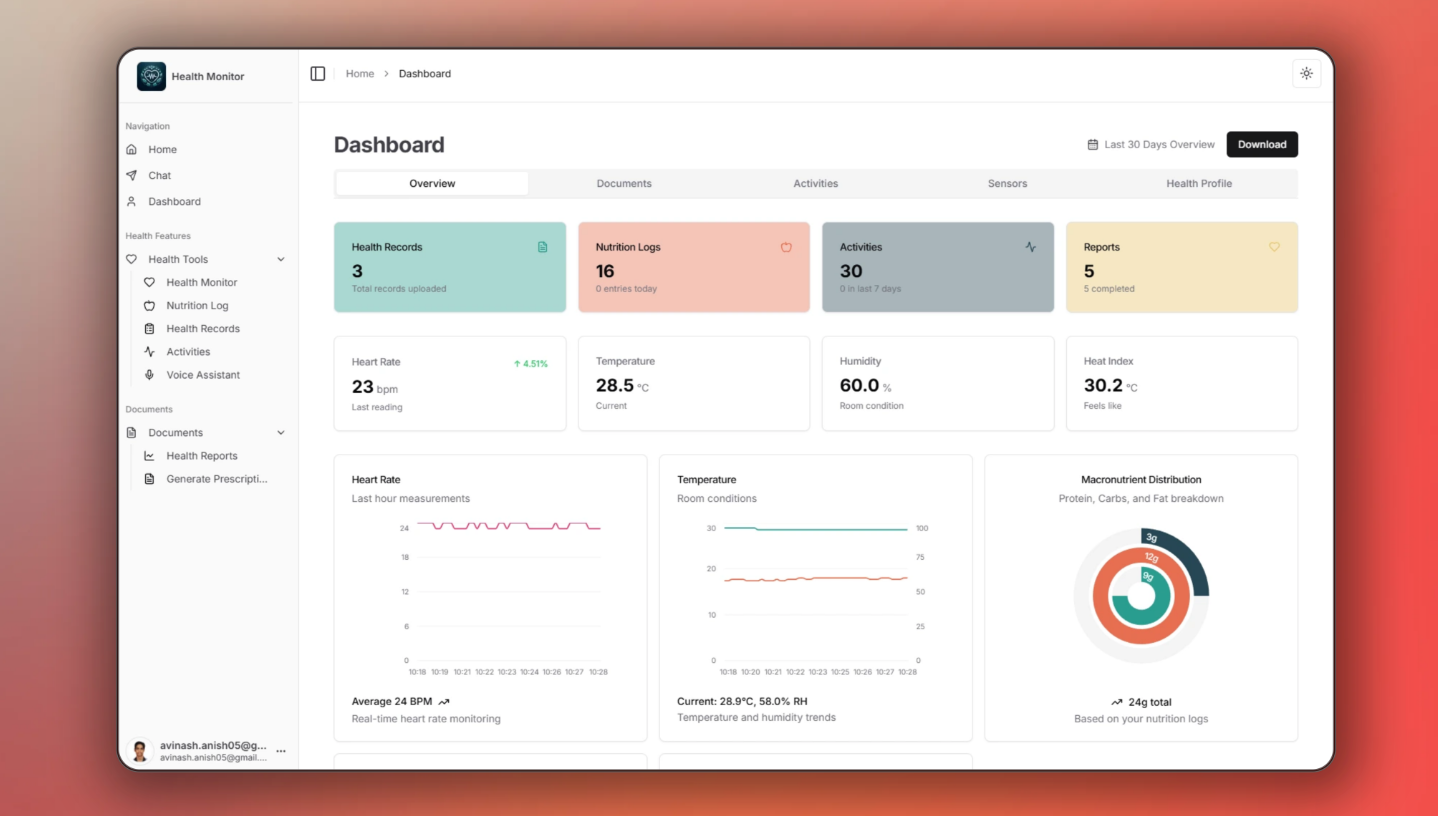
\includegraphics[width=0.9\columnwidth]{figures/hm-dashboard.png} % User to confirm/update path
\caption{The HealthHub main dashboard, providing a central point for users to view their health summary and access features.}
\label{fig:hm-dashboard}
\end{figure}

HealthHub supports multiple modalities for interacting with its AI assistant. Figure \ref{fig:hm-chat} illustrates the text-based chat interface. Furthermore, an integrated AI Voice and Video Assistant, shown in Figure \ref{fig:hm-video-assistant}, allows users to engage in spoken conversations and receive visual feedback from an AI avatar, enhancing the interactive experience.

\begin{figure}[!t]
\centering
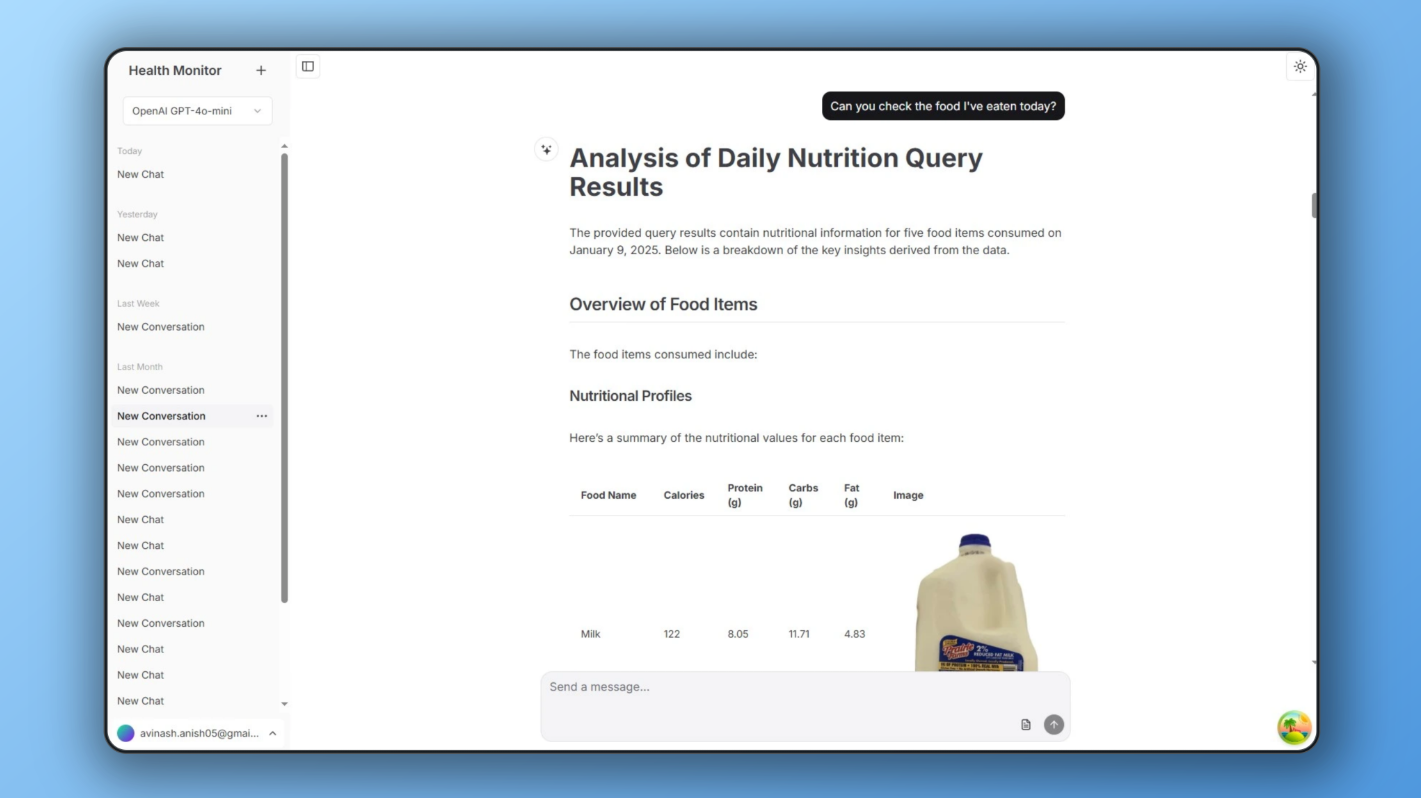
\includegraphics[width=0.9\columnwidth]{figures/hm-chat.png} % User to confirm/update path
\caption{HealthHub's text chat interface for querying the AI assistant about food safety, FSSAI guidelines, and nutrition.}
\label{fig:hm-chat}
\end{figure}

\begin{figure}[!t]
\centering
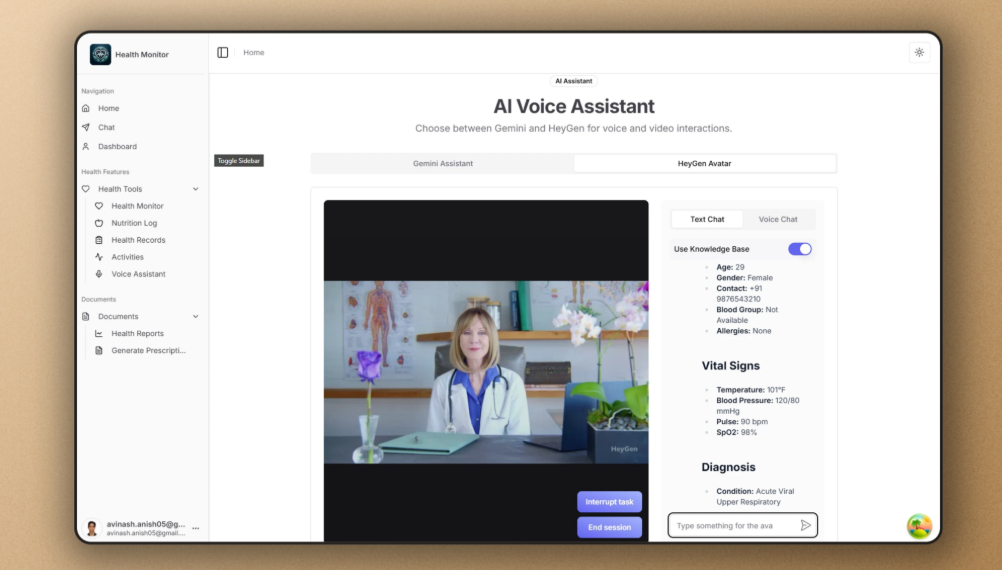
\includegraphics[width=0.8\columnwidth]{figures/hm-video.png} % Changed from 0.7, user to confirm filename (hm-video.png or specific AI assistant image)
\caption{The HealthHub AI Voice and Video Assistant interface, enabling spoken interaction and visual feedback.}
\label{fig:hm-video-assistant}
\end{figure}

\subsection{AI-Powered Food Safety and Nutritional Analysis}
Our AI core, combining a RAG pipeline and an SQL agent, demonstrated its ability to provide relevant and personalized information. Table \ref{tab:rag-examples} presents illustrative examples of the RAG pipeline addressing FSSAI and food safety queries.

\begin{table}[!ht]
\centering
\caption{Illustrative FSSAI & Food Safety Queries (RAG Pipeline)}
\label{tab:rag-examples}
\begin{tabular}{|p{0.4\columnwidth}|p{0.5\columnwidth}|}
\hline
\textbf{User Query/Scenario} & \textbf{HealthHub Response (Illustrative)} \\
\hline
User types: "Are there FSSAI rules for using artificial sweeteners in baked goods?" & Yes, FSSAI's Food Safety and Standards (Food Products Standards and Food Additives) Regulations, 2011, specify approved artificial sweeteners like Aspartame and Sucralose for use in baked goods, within prescribed maximum limits. For example, Aspartame is permitted up to 1000 mg/kg in certain bakery products. It's important to check product labels for declarations. \\
\hline
User asks: "What does FSSAI say about pesticide residues in fruits?" & FSSAI has established Maximum Residue Limits (MRLs) for various pesticides in different food commodities, including fruits, under the Food Safety and Standards (Contaminants, Toxins and Residues) Regulations, 2011. These limits are regularly reviewed. For specific fruits, it's best to refer to the latest FSSAI notifications on MRLs. \\
\hline
\end{tabular}
\end{table}

Table \ref{tab:sql-agent-examples} showcases the SQL agent processing natural language queries against logged dietary data.

\begin{table}[!ht]
\centering
\caption{Illustrative Personalized Nutritional Insights (SQL Agent)}
\label{tab:sql-agent-examples}
\begin{tabular}{|p{0.4\columnwidth}|p{0.5\columnwidth}|}
\hline
\textbf{User Query/Scenario} & \textbf{HealthHub Response (Illustrative)} \\
\hline
User asks via voice: "HealthHub, what was my average daily sugar intake this past week?" & Based on your logged food items from the past week, your average daily sugar intake was approximately 65 grams. The World Health Organization recommends adults consume no more than 25-50 grams of free sugars per day for optimal health. \\
\hline
User types: "Compare my protein intake yesterday with the day before." & Yesterday, your protein intake was 70g. The day before, it was 55g. You consumed 15g more protein yesterday. \\
\hline
\end{tabular}
\end{table}

\subsection{Sensor Data Integration and Alert Potential}
The sensor subsystem successfully logged physiological data (e.g., heart rate, SpO2 from MAX30102) to the user's profile. This data enables correlational analysis, as illustrated in Table \ref{tab:sensor-alert-example}.

\begin{table}[!ht]
\centering
\caption{Illustrative Sensor Data Correlation and Advisory}
\label{tab:sensor-alert-example}
\begin{tabular}{|p{0.4\columnwidth}|p{0.5\columnwidth}|}
\hline
\textbf{System Trigger/Scenario} & \textbf{HealthHub Advisory (Illustrative)} \\
\hline
User logs consumption of a highly caffeinated energy drink. System correlates this with sensor data showing a heart rate increase from baseline 70 bpm to 105 bpm, sustained for 45 minutes. & Noticed a significant heart rate increase after your logged energy drink. Frequent high caffeine intake can impact cardiovascular health. Consider moderation. \\
\hline
\end{tabular}
\end{table}

\subsection{System Performance and Responsiveness}
Initial evaluations indicate that HealthHub is responsive. Queries to the RAG pipeline for FSSAI information were typically answered within 3-5 seconds. The SQL agent also demonstrated efficient query execution for nutritional summaries, usually taking less than 2 seconds. While formal benchmarking is ongoing, the current performance supports an engaging user experience. 

\begin{appendices}
\chapter{Code and Acronyms}
% Appendix: Code, Acronyms

\section{Source Code}

The primary source code for the HealthHub project is hosted on GitHub:
\begin{itemize}
    \item Frontend (Next.js): \url{https://github.com/CubeStar1/health-monitor-next}
    \item Backend (Python/FastAPI): \url{https://github.com/CubeStar1/health-monitor-api}
\end{itemize}

\section{Acronyms}
\begin{itemize}
    \item AI: Artificial Intelligence
    \item API: Application Programming Interface
    \item CSS: Cascading Style Sheets
    \item DB: Database
    \item ECG: Electrocardiogram
    \item ESP8266: A Wi-Fi microchip
    \item GPT: Generative Pre-trained Transformer
    \item HTTP: Hypertext Transfer Protocol
    \item IoT: Internet of Things
    \item IR: Infrared
    \item JSON: JavaScript Object Notation
    \item LED: Light Emitting Diode
    \item LLM: Large Language Model
    \item ML: Machine Learning
    \item MQTT: Message Queuing Telemetry Transport
    \item NLP: Natural Language Processing
    \item OCR: Optical Character Recognition
    \item PDF: Portable Document Format
    \item RAG: Retrieval Augmented Generation
    \item RLS: Row-Level Security
    \item SpO2: Saturation of Peripheral Oxygen
    \item SQL: Structured Query Language
    \item UI: User Interface
    \item URL: Uniform Resource Locator
    \item UX: User Experience
\end{itemize}

\end{appendices}

\section{References}

[1] M. Alkhalaf, P. Yu, M. Yin, and C. Deng, "Applying generative AI with retrieval-augmented generation to summarize and extract key clinical information from electronic health records," Journal of Biomedical Informatics, p. 104662, 2024.

[2] T. Searle, Z. Ibrahim, J. Teo, and R. J. B. Dobson, "Discharge summary hospital course summarization of inpatient electronic health record text with clinical concept-guided deep pre-trained transformer models," Journal of Biomedical Informatics, p. 104358, 2023.

[3] S. Sai et al., "Generative AI for transformative healthcare: A comprehensive study of emerging models, applications, case studies, and limitations," IEEE Access, vol. 12, pp. 31078-31106, 2024.

[4] S. Reddy, "Generative AI in healthcare: An implementation science-informed translational path on application, integration, and governance," Implementation Science, vol. 19, p. 27, 2024.

[5] P. Zhang and M. N. Kamel Boulos, "Generative AI in medicine and healthcare: Promises, opportunities, and challenges," Future Internet, vol. 15, no. 9, p. 286, 2023.

[6] Leveraging generative AI models for synthetic data generation in healthcare: Balancing research and privacy, in 2023 International Conference on Smart Applications, Communications and Networking (SmartNets), 2023.

[7] W. Saba, S. Wendelken, and J. Shanahan, "Question-answering-based summarization of electronic health records using retrieval-augmented generation," arXiv preprint arXiv:2401.01469, 2024.

[8] Redefining medicine: The power of generative AI in modern healthcare, in 2024 5th International Conference on Smart Electronics and Communication (ICOSEC), 2024.

[9] D. S. W. Ting et al., "Retrieval-augmented generation for large language models and its generalizability in assessing medical fitness," arXiv preprint arXiv:2410.08431, 2024.

[10] L. M. Amugongo et al., "Retrieval-augmented generation for large language models in healthcare: A systematic review," Preprints, 2024.

[11] A. Bora and H. Cuayáhuitl, "Systematic analysis of retrieval-augmented generation-based LLMs for medical chatbot applications," Machine Learning and Knowledge Extraction, vol. 6, pp. 2355–2374, 2024.

[12] E. Albaroudi, T. Mansouri, and A. Alameer, "The intersection of generative AI and healthcare: Addressing challenges to enhance patient care," in 2024 Seventh International Women in Data Science Conference (WiDS PSU), 2024.

[13] Y. Xu, "The investigation of the application of RAG technology in the field of EHR," Science and Technology of Engineering, Chemistry and Environmental Protection, 2024.

[14] C. Troy, S. Sturley, J. M. Alcaraz-Calero, and Q. Wang, "Enabling generative AI to produce SQL statements: A framework for the auto-generation of knowledge based on EBNF context-free grammars," IEEE Access, vol. 11, pp. 123543-123564, 2023.

[15] P. Omrani et al., "Hybrid retrieval-augmented generation approach for LLMs query response enhancement," in 2024 10th International Conference on Web Research (ICWR), 2024.

[16] G. Papanastasiou, N. Dikaios, J. Huang, C. Wang, and G. Yang, "Is attention all you need in medical image analysis? A review," IEEE Journal of Biomedical and Health Informatics, vol. 28, no. 3, pp. 1398-1411, 2024. 

\end{document} 